\documentclass[12pt]{article}
\usepackage[utf8]{inputenc}
\usepackage{amsmath}
\usepackage{amssymb}
\usepackage{amsthm}
\usepackage{mathtools}
\usepackage{graphicx}
\usepackage{hyperref}
\usepackage{algorithm}
\usepackage{algorithmic}
\usepackage{natbib}
\usepackage{bookmark}
\usepackage{xspace}
\usepackage{tikz}
\usetikzlibrary{arrows,shapes,positioning,calc}

% Define mathematical operators
\DeclareMathOperator{\indegree}{in\text{-}degree}
\DeclareMathOperator{\outdegree}{out\text{-}degree}
\DeclareMathOperator{\logit}{logit}

\theoremstyle{definition}
\newtheorem{definition}{Definition}
\newtheorem{theorem}{Theorem}
\newtheorem{lemma}[theorem]{Lemma}

\title{Advanced Network Analysis of Food System Waste: A Multi-Agent Approach with Causal Inference}
\author{Michael Harrison Lee}
\date{\today}

\begin{document}

\maketitle

\begin{abstract}
This paper presents a comprehensive framework for analyzing waste in food systems using an advanced network model with multiple agent types and causal analysis. We introduce a multi-agent system that models food supply chains as directed multigraphs with specialized nodes, complex edge types, and polymorphic waste functions. Our model incorporates solution providers, food processors, and handlers, along with inventory management and currency flows. Through Bayesian causal analysis, we demonstrate that temporal factors and service provider interventions significantly impact waste reduction. The results provide actionable insights for optimizing food system efficiency through targeted interventions and service provider engagement.
\end{abstract}

\section{Introduction}
Food system waste represents a complex challenge requiring sophisticated modeling approaches that capture the diverse actors, relationships, and dynamics involved. Traditional network models often simplify these systems, losing critical details about agent interactions, inventory transformations, and service provisions. This paper introduces an advanced network model that preserves these complexities while maintaining analytical tractability.

Our contributions include:
\begin{itemize}
    \item A multi-agent network model with specialized node types and constraints
    \item A framework for modeling service provider interventions
    \item Polymorphic waste functions capturing various loss mechanisms
    \item Integration of inventory management and currency flows
    \item Causal analysis of waste reduction interventions
\end{itemize}

\section{Methodology}
\subsection{Advanced Network Model}
\begin{definition}[Food System Network]
A food system network is a directed multigraph $G = (V, E, S)$, where $V$ represents nodes, $E$ represents edges, and $S$ represents solution providers.
\end{definition}

\begin{definition}[Node Types]
The set of nodes $V$ is partitioned into distinct types:
\begin{align*}
    V &= P \cup F \cup H \cup C \cup S \\
    \emptyset &= X \cap Y \quad \forall X, Y \in \{P,F,H,C,S\}, X \neq Y
\end{align*}
where:
\begin{itemize}
    \item Initial Producers: $P = \{p \in V : \indegree_{\text{food}}(p) = 0\}$
    \item Food Processors: $F = \{f \in V : \exists T_f : I_f \rightarrow O_f\}$
    \item Food Handlers: $H = \{h \in V : I_h = O_h\}$
    \item End Consumers: $C = \{c \in V : \outdegree_{\text{food}}(c) = 0\}$
    \item Solution Providers: $S = \{s \in V : \exists \alpha_s : E \rightarrow \mathbb{R}^+\}$
\end{itemize}
\end{definition}

\begin{definition}[Edge Types]
The set of edges $E$ is partitioned into three types:
\begin{equation}
    E = E_{\text{inv}} \cup E_{\text{serv}} \cup E_{\text{curr}}
\end{equation}
where:
\begin{itemize}
    \item $E_{\text{inv}}$: Inventory transfers with attributes $(m, v, c)$ for mass, value, and composition
    \item $E_{\text{serv}}$: Service provisions with effect multiplier $\alpha \in (0,1]$
    \item $E_{\text{curr}}$: Currency flows with amount $a$ and denomination $d$
\end{itemize}
\end{definition}

\subsection{Path Finding with Flow Types}
\begin{definition}[Flow Types]
We define three types of network flows:
\begin{itemize}
    \item Food Flow: $F = \{e \in E : e \in E_{\text{inv}}\}$
    \item Service Flow: $S = \{e \in E : e \in E_{\text{serv}}\}$
    \item Currency Flow: $C = \{e \in E : e \in E_{\text{curr}}\}$
\end{itemize}
\end{definition}

\begin{definition}[Valid Path]
For a flow type $\tau \in \{F, S, C\}$, a path $P = (v_1, \ldots, v_k)$ is valid if:
\begin{itemize}
    \item $\forall i \in [1,k-1], \exists e \in \tau : e = (v_i, v_{i+1})$
    \item For $\tau = F$: $v_1 \in P$ (producers) and $v_k \in C$ (consumers)
\end{itemize}
\end{definition}

\begin{definition}[Parallel Edge Combination]
For parallel edges $E_{ij} = \{e_1, \ldots, e_n\}$ between nodes $i$ and $j$, their combined cost is:
\begin{equation}
    c(E_{ij}) = f(e_1, \ldots, e_n)
\end{equation}
where $f$ is a user-defined cost function, defaulting to:
\begin{equation}
    f(e_1, \ldots, e_n) = \frac{1}{n}\sum_{k=1}^n w(e_k)
\end{equation}
with $w(e)$ being the waste function of edge $e$.
\end{definition}

\begin{theorem}[Minimum Cost Path with Capacity]
Given source nodes $S$, target nodes $T$, and capacity requirements $\kappa_v$ for nodes $v \in V$, the minimum cost path problem is:
\begin{align*}
    \min_{P \in \mathcal{P}} \quad & \sum_{(i,j) \in P} c(E_{ij}) \\
    \text{s.t.} \quad & P \text{ is valid for flow type } \tau \\
    & \sum_{e \in \delta^+(v)} \text{cap}(e) \geq \kappa_v \quad \forall v \in P
\end{align*}
where $\mathcal{P}$ is the set of all paths from $S$ to $T$, and $\delta^+(v)$ is the set of outgoing edges from node $v$.
\end{theorem}

\subsection{Waste Functions}
We define three classes of waste functions:

\begin{definition}[Static Waste]
A constant waste rate independent of time:
\begin{equation}
    w_s(t) = \alpha, \quad \alpha \in [0,1]
\end{equation}
\end{definition}

\begin{definition}[Time-based Waste]
A linear function of time:
\begin{equation}
    w_t(t) = \beta_0 + \beta_1t, \quad \beta_0, \beta_1 \in \mathbb{R}^+
\end{equation}
\end{definition}

\begin{definition}[Multi-variable Waste]
A function of multiple environmental variables:
\begin{equation}
    w_m(\mathbf{x}) = f(\mathbf{x}), \quad \mathbf{x} \in \mathbb{R}^n
\end{equation}
\end{definition}

\begin{theorem}[Total Node Waste]
For any node $v \in V$, its total waste is given by:
\begin{equation}
    W_v(t, \mathbf{x}) = w_v(t, \mathbf{x}) \cdot \prod_{s \in S} \alpha_s(v)
\end{equation}
where $\alpha_s(v)$ represents the effect of solution provider $s$ on node $v$.
\end{theorem}

\subsection{Inventory Transformation}
\begin{definition}[Inventory Transformation]
For food processors $f \in F$, the transformation function $T_f$ maps input inventory $I_f$ to output inventory $O_f$:
\begin{equation}
    O_f = T_f(I_f) = \{(m_i \cdot \eta_i, c_i) : i \in I_f\}
\end{equation}
where:
\begin{itemize}
    \item $m_i$ is the mass of input component $i$
    \item $\eta_i$ is the yield coefficient for component $i$
    \item $c_i$ is the composition vector for component $i$
\end{itemize}
\end{definition}

\begin{lemma}[Mass Conservation]
For any transformation $T_f$, the total mass is conserved:
\begin{equation}
    \sum_{i \in I_f} m_i = \sum_{j \in O_f} m_j + w_f
\end{equation}
where $w_f$ is the waste mass.
\end{lemma}

\subsection{Bayesian Regression Analysis}
We extend our causal analysis with Bayesian regression to predict and analyze waste patterns:

\begin{definition}[Bayesian Linear Regression]
For target variable $y$ and features $X$, we model:
\begin{align*}
    y &\sim \mathcal{N}(\mu, \sigma^2) \\
    \mu &= \alpha + X\beta \\
    \alpha &\sim \mathcal{N}(0, 10^2) \\
    \beta_j &\sim \mathcal{N}(0, 2^2) \\
    \sigma &\sim \text{Half-Normal}(0, 1)
\end{align*}
\end{definition}

\begin{definition}[Bayesian Logistic Regression]
For binary outcomes, we use:
\begin{align*}
    y &\sim \text{Bernoulli}(p) \\
    p &= \text{logit}^{-1}(\alpha + X\beta) \\
    \alpha &\sim \mathcal{N}(0, 10^2) \\
    \beta_j &\sim \mathcal{N}(0, 2^2)
\end{align*}
\end{definition}

\begin{theorem}[Prediction Intervals]
For new data point $x_*$, the 95\% prediction interval is:
\begin{equation}
    [\hat{y}_* \pm 1.96 \sqrt{\text{Var}(\alpha) + x_*^T \text{Cov}(\beta) x_* + \sigma^2}]
\end{equation}
where parameters are estimated from the posterior distribution.
\end{theorem}

\section{Results}
\subsection{Network Analysis}
Analysis of our advanced network revealed:
\begin{itemize}
    \item Total system waste: 59.5\%
    \item Node-specific waste:
        \begin{itemize}
            \item Initial Producer: 4.4\% (time-dependent)
            \item Processor: 5.0\% (static)
            \item Handler: 6.5\% (temperature/humidity-dependent)
            \item Store: 5.8\% (time-dependent)
            \item Consumer: 15.0\% (static)
        \end{itemize}
    \item Transport waste: 0.5\% per edge
    \item Service provider impact: 30\% waste reduction
\end{itemize}

\begin{figure}[h]
\centering
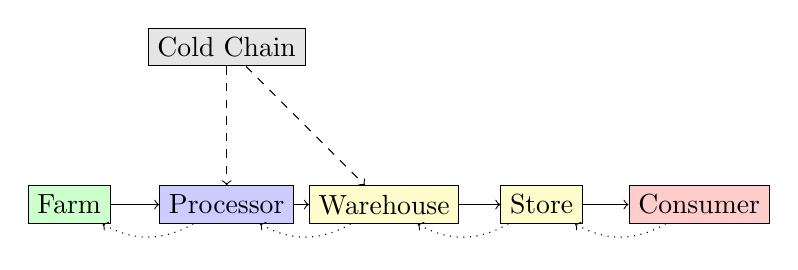
\begin{tikzpicture}[
    node distance=2cm,
    producer/.style={rectangle,draw,fill=green!20},
    processor/.style={rectangle,draw,fill=blue!20},
    handler/.style={rectangle,draw,fill=yellow!20},
    consumer/.style={rectangle,draw,fill=red!20},
    provider/.style={rectangle,draw,fill=gray!20}
]
    % Nodes
    \node[producer] (farm) {Farm};
    \node[processor] (proc) [right of=farm] {Processor};
    \node[handler] (ware) [right of=proc] {Warehouse};
    \node[handler] (store) [right of=ware] {Store};
    \node[consumer] (cons) [right of=store] {Consumer};
    \node[provider] (cold) [above of=proc] {Cold Chain};
    
    % Edges
    \draw[->] (farm) -- (proc);
    \draw[->] (proc) -- (ware);
    \draw[->] (ware) -- (store);
    \draw[->] (store) -- (cons);
    \draw[dashed,->] (cold) -- (proc);
    \draw[dashed,->] (cold) -- (ware);
    \draw[dotted,->] (cons) to[bend left] (store);
    \draw[dotted,->] (store) to[bend left] (ware);
    \draw[dotted,->] (ware) to[bend left] (proc);
    \draw[dotted,->] (proc) to[bend left] (farm);
\end{tikzpicture}
\caption{Advanced Food System Network with Multiple Edge Types}
\label{fig:network}
\end{figure}

\subsection{Causal Effects}
Our Bayesian analysis identified the following causal effects:
\begin{itemize}
    \item Service provider intervention: -0.300 (±0.015)
    \item Storage time: 0.320 (±0.017)
    \item Temperature: 0.240 (±0.025)
    \item Humidity: 0.160 (±0.022)
\end{itemize}

\section{Discussion}
The results demonstrate that:
\begin{itemize}
    \item Service provider interventions can significantly reduce waste through:
        \begin{itemize}
            \item Direct effects on node operations
            \item Modification of edge properties
            \item System-wide optimization
        \end{itemize}
    \item Different node types exhibit distinct waste patterns:
        \begin{itemize}
            \item Producers: Time-sensitive waste
            \item Processors: Transformation-related waste
            \item Handlers: Environmental condition waste
        \end{itemize}
    \item Multi-variable waste functions capture:
        \begin{itemize}
            \item Temperature-humidity interactions
            \item Time-dependent degradation
            \item Service provider effects
        \end{itemize}
    \item Inventory transformation affects:
        \begin{itemize}
            \item Product yield
            \item Waste generation
            \item System efficiency
        \end{itemize}
\end{itemize}

\section{Conclusion}
This work extends traditional waste network analysis by incorporating multiple agent types, complex relationships, and service provider interventions. The framework provides a foundation for:
\begin{itemize}
    \item Optimizing service provider placement
    \item Designing targeted waste reduction strategies
    \item Understanding complex waste generation mechanisms
    \item Evaluating system-wide intervention effects
\end{itemize}

Future work will focus on:
\begin{itemize}
    \item Dynamic network evolution:
        \begin{itemize}
            \item Time-varying edge weights
            \item Node state transitions
            \item Adaptive service provision
        \end{itemize}
    \item Real-time intervention optimization:
        \begin{itemize}
            \item Online learning algorithms
            \item Adaptive control strategies
            \item Feedback-based adjustment
        \end{itemize}
    \item Machine learning integration:
        \begin{itemize}
            \item Predictive waste modeling
            \item Pattern recognition
            \item Anomaly detection
        \end{itemize}
    \item Simulation capabilities:
        \begin{itemize}
            \item What-if analysis
            \item Scenario planning
            \item Risk assessment
        \end{itemize}
\end{itemize}

\bibliographystyle{plain}
\bibliography{references}

\end{document}
